%% Benutzerdefinierte Kommandos

	\newcommand{\todo}[1]{\colorbox{red}{\textcolor{white}{TODO: #1}}}
	


%% Pakete 

\documentclass[a4paper, 12pt]{scrartcl}
\usepackage{ucs}
\usepackage[utf8x]{inputenc}
\usepackage[T1]{fontenc}
\usepackage[english,ngerman]{babel}
\usepackage{graphicx}
\usepackage{enumerate}
\usepackage{color}
\usepackage{xcolor}
\usepackage{amsfonts}
\usepackage{amsmath}
\usepackage{scrtime} % for \thistime
\usepackage{dsfont} %for \mathds
\usepackage{framed}
\usepackage[colorlinks=true,urlcolor=blue,linkcolor=black]{hyperref}
\usepackage{perpage} %the perpage package, used for footnotes
\usepackage{pifont} %used for customized footnotes
\usepackage{caption}
\usepackage{float}
\usepackage{mathrsfs}
\usepackage[usestackEOL]{stackengine}


\makeatletter 
\renewcommand\paragraph{\@startsection{paragraph}{4}{\z@}% 
  {-3.25ex\@plus -1ex \@minus -.2ex}% 
  {1.5ex \@plus .2ex}% 
  {\normalfont\normalsize\bfseries}} 
\makeatother
\setlength{\parindent}{0pt}
    
\begin{document}

\begin{normalsize}

\raggedright\textbf{\Huge Peketeinräumerding}\\	
		\begin{flushright}
		\textit{Michael Thomas}
		\textit{Andreas Glatz}
		\textit{Simon Weitzel}
		\textit{Felix Baral-Weber}\\
		Stand: \space \today \space \thistime
		\end{flushright}

\end{normalsize}
\tableofcontents
\section{Einführung}
\subsection{Zweck des Dokuments}
Dieses Dokument beschreibt die Anforderungen und Implementierungsdetails an eine Echtzeitsystemanwendung die das Abschlussprojekt des Moduls Echtzeitbetriebssysteme der EAH Jena. Dieses Dokument richtet sich dabei an den Vorgaben für ein Software Requirements Specification (SRS) nach dem \href{https://de.wikipedia.org/wiki/Software_Requirements_Specification}{IEEE Standard 830-1998}. Der Modulverantwortliche ist Prof Dr. Oliver Jack aus dem Fachbereich Elektrotechnik und Informationstechnik.\\

\subsection{Einstieg in die Projektphase}
Die Arbeit an der Programmumsetzung wurde in die Teilbereiche Hochregal-Steuerung, Simulation, Integritätsprüfung und User-Input und Visualisierung aufgeteilt um diese Bereiche allein bzw. in Gruppen parallel  abarbeiten zu können.\\
Dabei ergab sich folgende Aufteilung:
\begin{itemize} 
	\item Hochregal-Steuerung $\rightarrow$ Michael Thomas, Simon Weitzel
	\item Simulation $\rightarrow$ Felix Baral-Weber, Andreas Glatz
	\item Integritätsprüfung und User-Input $\rightarrow$ Simon Weitzel, Michael Thomas
	\item Visualisierung $\rightarrow$ Andreas Glatz, Felix Baral-Weber
\end{itemize}

Desweiteren wurden Hauptverantwortliche für alle Teilbereich des Projekt festgelegt.\\

Die da wären:\\
\begin{itemize} 
	\item Michael Thomas: Programmumsetzung
	\item Andreas Glatz: Tests
	\item Simon Weitzel: Strukturierte Analyse
	\item Felix Baral-Weber: Latex-Template und Funktionale Anforderung
\end{itemize}
\section{Allgemeine Beschreibung}
\subsection{Aufgabenstellung und Umsetzungsansatz}
Die Aufgabestellung des Semesterprojektes ist es eine Hochregallagersimulation unter zuhilfenahme eines Echtzeitbetriebssystems zu erstellen. Diese soll das gesamte System mit einer statisch gewählten Regaldimension sowohl steuern als auch simulieren.
Das Simulationmodell umfasst ein Regallagersystem mit $5*10$ Regalfächern, ein Ein- und ein Ausgabeslot und einen Turm zum be- und entladen. Dieser Turm ist auf einer Achse montiert auf welcher er sich in X-Richtung bewegen kann, desweiteren kann der Ausleger am Turm in Y-Richtung herauf und herab und in Z-Richtung rein und raus gefahren werden. Diese Bewegungen und die daraus resultierende Position des Turms werden von Tastern auf der Schiene ermittelt.\\
Auf der X-Achse und auf der Y-Achse sind jeweils 10 Taster und auf der Z-Achse 3.

Dem Anwender steht als Eingabe- und Ausgabemedium die Konsole zur Verfügung.
\newline\newline
Ihm stehen folgende Befehle zur Verfügung:
\begin{itemize} 
	\item getspace $\rightarrow$ Zeigt aktuelle Belegung des Hochregallagers an
	\item vsetspace[x][y] $\rightarrow$ Definiert einen Platz als schon belegt
	\item clearspace[x][y] $\rightarrow$ Definiert einen Platz als frei
	\item insert[x][y] $\rightarrow$ Holt ein Klötzchen vom Eingabe-Slot und legt es an gewünschter Position im Hochregallager ab
	\item remove[x][y] $\rightarrow$ Holt ein Klötuchen von der gewünschten Position ab und legt es an den Ausgabe-Slot
\end{itemize}

Sollte ein Befehl nicht möglich sein, da zum Beispiel ein Hochregallagerplatz oder der Ausgabe-Slot bereits belegt ist, wird der Anwender durch eine Fehlermeldung in der Konsole darauf aufmerksam gemacht und der Befehl nicht ausgeführt.

Die Visualisierung des Hochregallagers erfolgt ebenfalls in der Konsole, in welcher sowohl das Hochregal und dessen Belegung als auch die Position des Turms und dessen Auslegers, durch ASCI-Zeichen stilisiert dargestellt werden.
Dabei liegt der Ursprung der Koordinaten und somit der Regalplatz (0,0) in der linken unteren Ecke.
Die Darstellung des Ein- und Ausfahren des Auslegers wird unterhalb dargestellt. Dabei stellt die linke Position den zum Ein-/Ausgabe-Slot gefahrenen Arm da, die rechte Position die in das Regal hereingefahrene.
\todo{Bild der Konsole einfügen}

\subsection{Entwicklungsumgebung und Programmierung}
Als Entwicklungs- und Testumgebung wurde Windriver Workbench 3.3 genutz und die Programmiersprache C verwendet.
Es wurden für das Echtzeitbetriebssystem Vxworks Libaries inkludiert.



\section{Spezifische Anforderungen}
\subsection{Funktionale Anforderungen}
\subsubsection{DFD1 Simulation}
\begin{figure}[H]
	\centering
  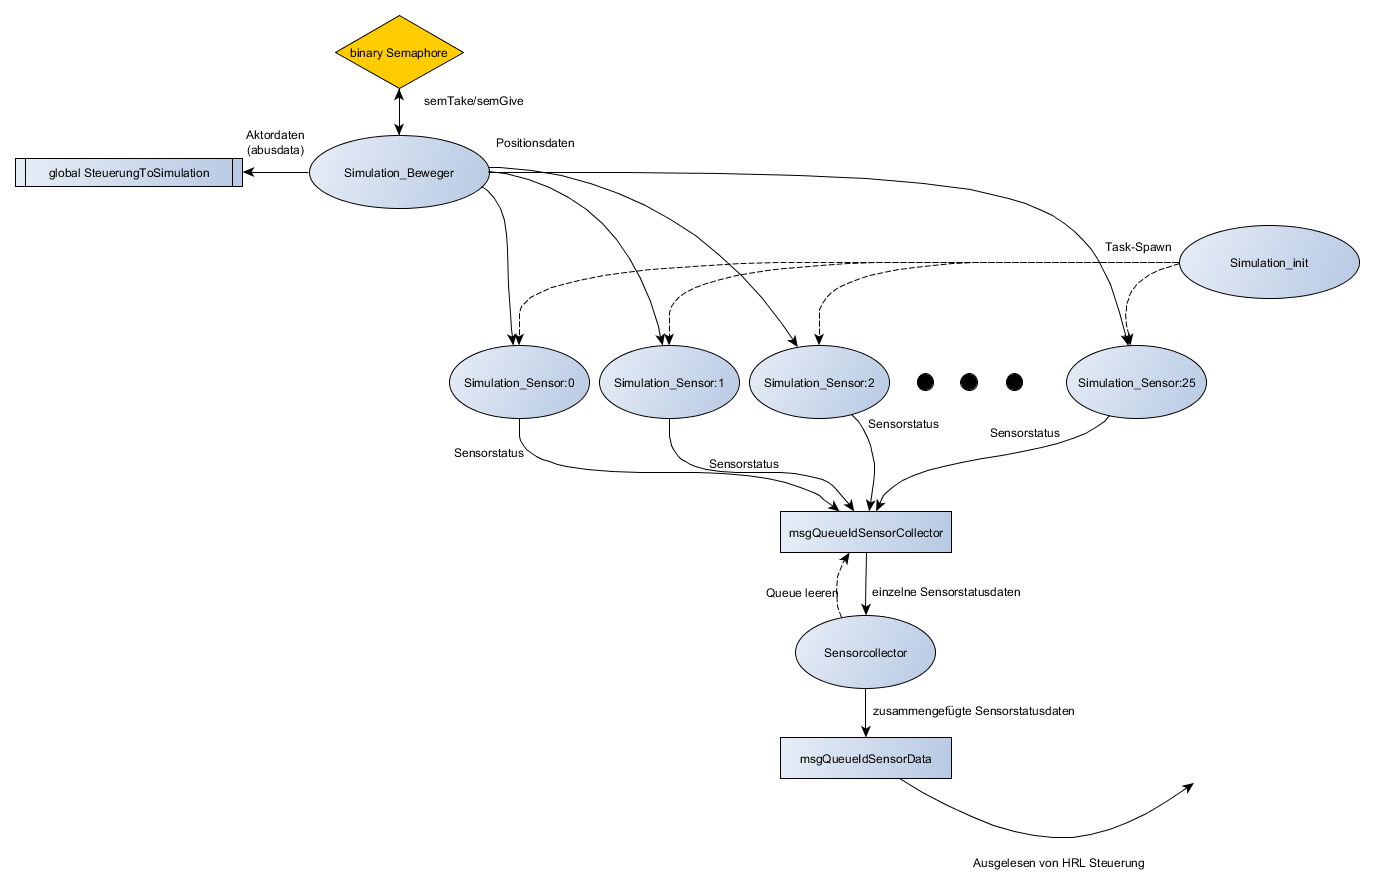
\includegraphics[width=\textwidth]{DFD/dfd1_simulation1_1.png}
	\caption{DFD1 Simulation}
	\label{fig1}
\end{figure}
\begin{figure}[H]
	\centering
  \includegraphics[width=\textwidth]{diagrams/gand.png}
	\caption{Gantt Diagramm der Task der Simulation}
	\label{gantt}
\end{figure}
\paragraph{Sensorcollector}
Der \textbf{Sensorcollector} sammelt aus der \textbf{MessageQueue} die Einträge aller Sensoren. Wenn ein Sensor ausfällt bleibt der Wert des Sensors auf 1.
%\input{lectures/lecture12}
\end{document}